
\subsubsection{Thermal Grooving}



\begin{figure}[h!]
	\centering
	\begin{subfigure}[c]{0.45\textwidth}
		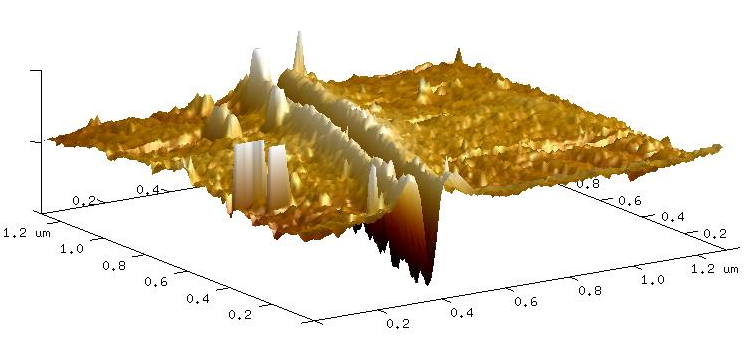
\includegraphics[width=\linewidth]{afm-groove-fega}
		\subcaption{~}
		\label{fig:afm-groove-fega}		
	\end{subfigure}
	\begin{subfigure}[c]{0.45\textwidth} 
		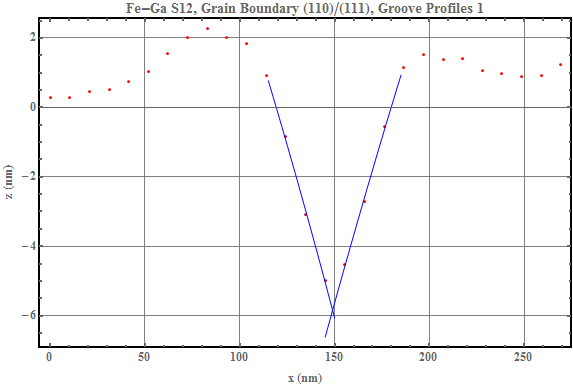
\includegraphics[width=\linewidth]{fega-groove-profile}
		\subcaption{~}
		\label{fig:fega-groove-profile}		
	\end{subfigure}
	\caption{(a) 3D rendering of (110)/(111) grain boundary on surface of  for (Fe-19\%Ga)+1.0\%NbC sample where the depth of groove is ~8 nm. (b) A quadratic fit of a (110)/(111) grain boundary profile for a (Fe-19\%Ga)+1.0\%NbC sample.}
	\label{fig:thermal-groove}
\end{figure}

\begin{table}[h!]
	\centering
	\caption{Calculated dihedral angles and relative energies from our most symmetric grain boundary groove.}
	\begin{tabular} { |p{1cm}||c|c|c|c|  } 
		\hline
		\multicolumn{5}{|c|}{fe-ga-s12-006 profile analysis - GB (110)/(111)}\\
		\hline
		~	&\multicolumn{2}{|c|}{Bruker Software}		&\multicolumn{2}{|c|}{Quadratic Fit}	\\
		\hline
		Profile	&Dihedral Angle (\degree)	&Relative GB Energy	&Dihedral Angle (\degree)	&Relative GB Energy \\ 
		\hline
		1		&156.957	&0.399471	&151.253	&0.496475	\\
		\hline
		2		&156.244	&0.411657	&157.093	&0.397144	\\
		\hline
		3		&154.402	&0.443063	&155.554	&0.423432	\\
		\hline
		4		&157.221	&0.394955	&152.785	&0.470541	\\
		\hline
		5		&154.732	&0.437445	&154.966	&0.433458	\\
		\hline
		6		&158.386	&0.375003	&154.482	&0.441706	\\
		\hline
		\textbf{Avg}	&156.324$\pm$1.52919	&0.410266$\pm$0.0261178	&154.356$\pm$2.06926	&0.443793$\pm$0.0351932\\
		\hline
	\end{tabular}
	\label{groove-analysis}
\end{table}


The thermal grooving technique was examined to provide a comparison point to our proposed gallium contact angle method.  These thermal grooves appear at grain boundaries, but the most information can be drawn from grain boundaries formed by two different crystal orientations. Using electron backscatter diffraction, EBSD, we identified grain orientations on samples of galfenol and alfenol to identify the grain boundaries where \hkl(100), \hkl(110), and \hkl(111) orientations met.  By measuring the dihedral angle formed at these grain boundaries after polishing and annealing, we calculated the ratio of grain boundary energy and surface energy according to the following equation: 
\begin{equation}
\frac{\gamma_{GB}}{\gamma_{S}} = 2\cos\left(\frac{\Psi_{S}}{2}\right) 
\end{equation}
where $\gamma_{GB}$ is the grain boundary energy, $\gamma_{S}  $ is the surface energy, and $\Psi_{S} $ is the dihedral angle, as described in Rohrer et al.\cite{Rohrer2010a} The most symmetric thermal groove came from a \hkl(110)/\hkl(111) grain boundary on a rolled and annealed (Fe-19\%Ga)+1.0\%NbC sample made by Suok-Min Na, as seen in the Figure \ref{fig:thermal-groove}.  The grain boundary profiles were measured using atomic force microscopy (AFM), and the dihedral angles were extrapolated from the profiles using both AFM software by Bruker and, the more accurate, quadratic fit.  The results are shown in Table \ref{groove-analysis}.  This groove in particular had a depth of $\sim$8 nm which is significantly smaller in depth compared to grooves of other metal alloys in literature.  Also, many of the grain boundary grooves were not suitable for measuring based on their lack of symmetry at the grain boundary interface. It is worthy to note that this technique is very time consuming and slightly destructive to the surface. To properly analyze the thermal grooving technique, an extensive grain boundary study of annealing temperatures and times on Alfenol and Galfenol would have to be carried out. While this may be an interesting avenue of research in the future, the resultant calculations of relative grain energies does not benefit our ultimate goal of achieving a comprehensive AGG model for Galfenol and Alfenol. Realization of our goal lies in the measurement of orientation-dependent surface energy using contact angle measurements. 
	


\subsubsection{Contact Angle Goniometer}
Preliminary designs of our contact angle goniometer implement a radiative temperature control box which encloses an argon gas filled container where the sample resides, as seen in Figure \ref{fig:rad-temp-box}.  The argon filled container was initially made of a clear acrylic plastic, but prolonged exposure to temperatures above 80\degree C caused thermal deformation of the plastic making longer experiments impossible to perform without environment contamination.  A clear pyrex container replaced the acrylic box to fix this issue.  Application of the liquid gallium drop to our surfaces was done via a mounted plastic syringe with commercially available disposable stainless steel hypodermic needles.  Observations of this application show that the hypodermic needles present multiple problems to the sessile drop method.  Liquid gallium tends to adhere strongly to the stainless steel needle tips which makes wetting to the sample very difficult.  Tapping the syringe will remove the drop from the needle and allow gallium to wet the surface, but this is not ideal because the additional dropping force from gravity will cause additional spreading not associated with the intrinsic surface energy of the substrate.  Also, the angled hypodermic tip tends to deform the highly viscous gallium drop resulting in non-uniform hemispheric drop shapes, as shown in Figure \ref{fig:deformed-ga}.
\begin{figure}
	\centering
	\begin{subfigure}[c]{0.45\textwidth}
		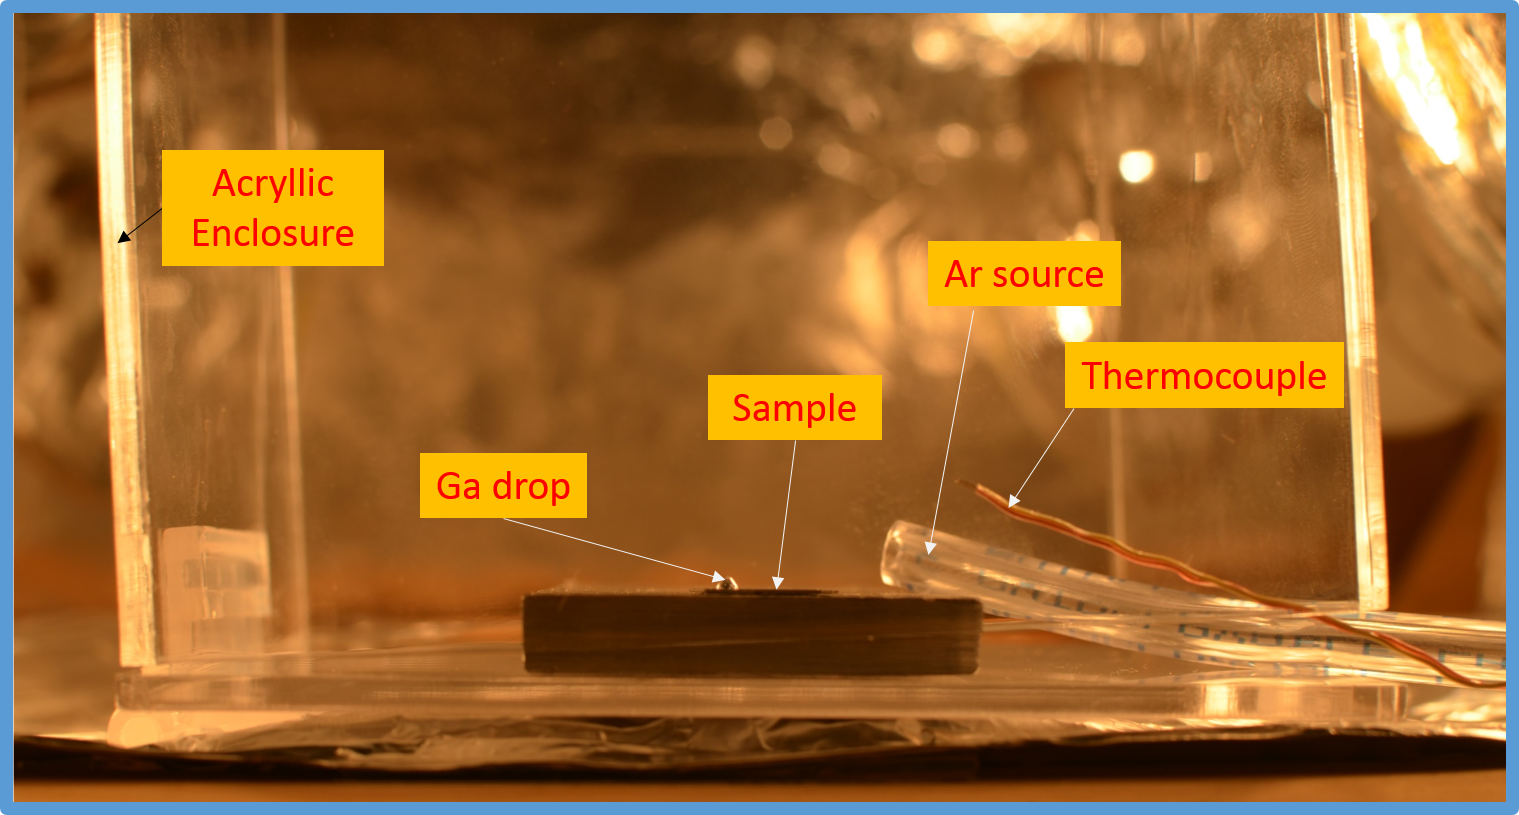
\includegraphics[width=\linewidth]{rad-temp-box}
		\subcaption{~}
		\label{fig:rad-temp-box}		
	\end{subfigure}
	\begin{subfigure}[c]{0.45\textwidth} 
		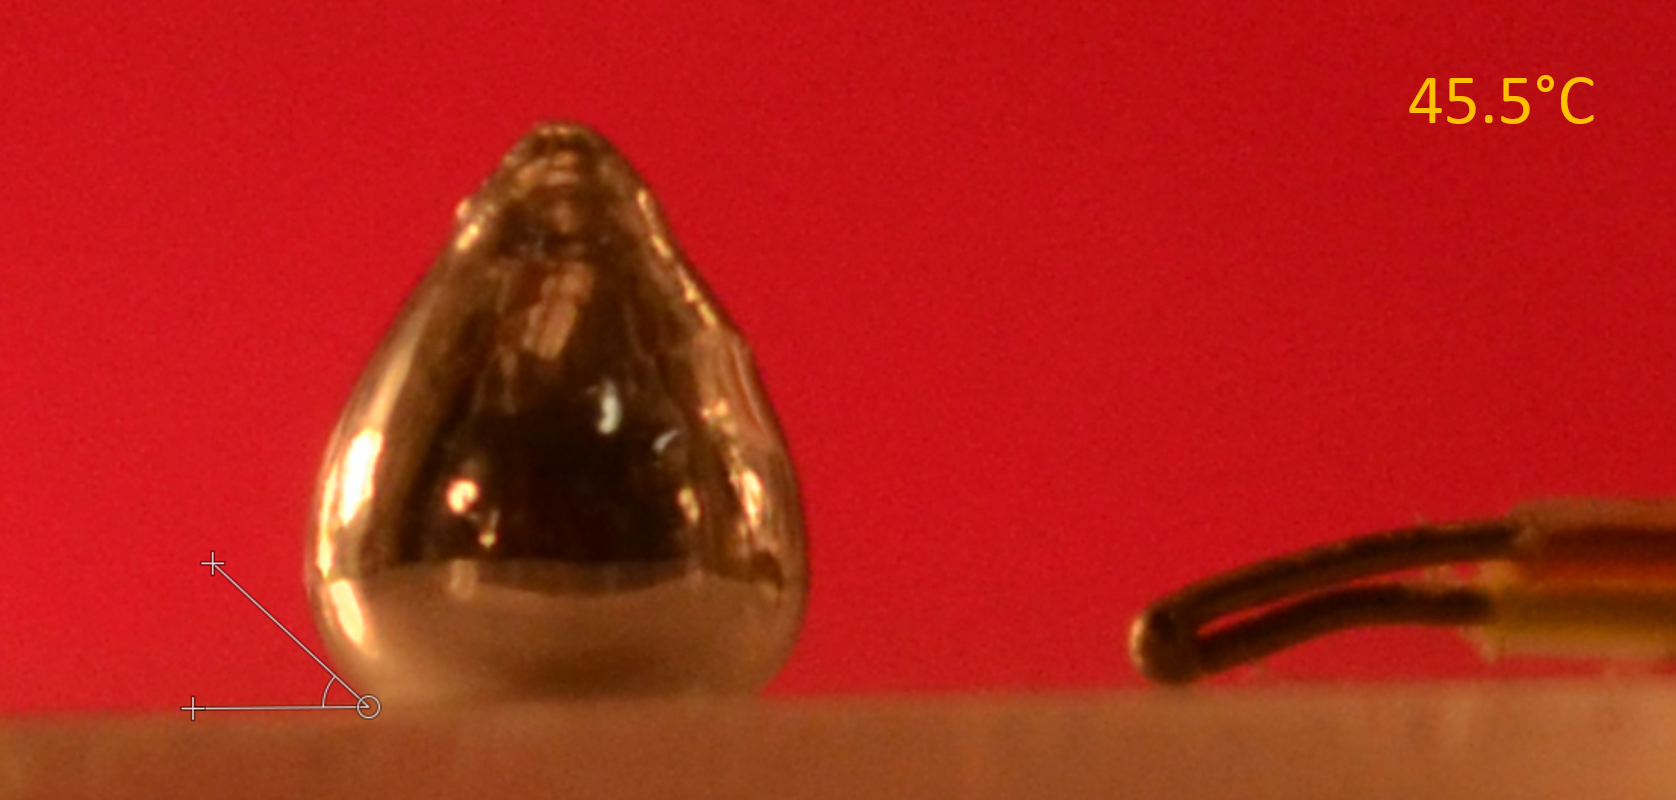
\includegraphics[width=\linewidth]{deformed-ga}
		\subcaption{~}
		\label{fig:deformed-ga}		
	\end{subfigure}
	\caption{(a) The first design of our contact angle goniometer.  The acrylic container houses the argon environment and sample.  This design was modified with a more stable glass enclosure. (b) A highly deformed gallium drop next to the thermocouple on a ceramic YAG test sample at 45.5\degree C.}
	\label{fig:prelim-design}
\end{figure}

For this experiment to succeed, a number of challenges were overcome. The simplest task involved polishing Galfenol samples using incrementally higher grit SiC paper and subsequent 0.1 $\mu$m colloidal silica particles to decrease the roughness to below 100 nm, as proven using AFM measurements. [FIND AFM PICTURE OF ROUGHNESS]

Gallium droplets must carefully wet the surface while forming an axisymmetric and spherical-like droplet on the solid surface. 

\begin{outline}[enumerate]
	\1 Radiative box [~]
		\2 Plexiglass chamber [X]
		\2 Glass chamber [X]
		\2 Low control of temperature and image clarity [~]
			\3 Need temperature control and backlighting, while improving gas environment. [~]
	\1 Aluminum conductive environmental chamber [~]
		\2 Deformed droplets persist and contact angle cannot be properly measured [~]
		\2 HCl etching to achieve axisymmetric gallium drops [~]
		\2 Surface energy can be measured [~]
	\1 MRS Fall Meeting [~]
		\2 Learning from wetting dynamics community [~]
			\3 Static contact angles are not well accepted due to inconsistency  [~]
			\3 make connections to wetting dynamics research group in UMD Mechanical Engineering [~] 
			\3 Learn that gallium drop model is incorrect on a thermodynamic equilibrium level [~]
				\4 Using one thermodynamic equilibrium equation and then plugging values into another thermodynamic equilibrium equation [~]
		
\end{outline}
